\chapter[SCP-013 蓝色女士香烟]{
    SCP-013 Blue Lady Cigarettes\\
    SCP-013 蓝色女士香烟
}

\label{chap:SCP-013}

\begin{figure}[H]
    \centering
    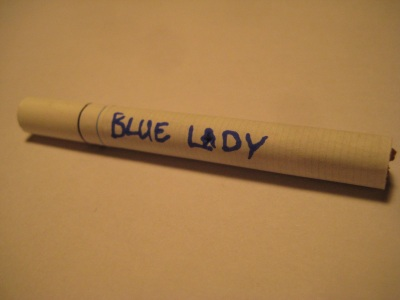
\includegraphics[width=0.5\linewidth]{images/SCP.013.jpg}
    \caption*{SCP-013}
\end{figure}

\bb{项目编号:}SCP-013

\bb{项目等级:}Safe

\bb{特殊收容措施:}SCP-013应保管于66号站点的安全储藏库。应监视受影响受试者症状间的区别。应每天与受影响受试者对话,并记录任何观念上的变化。

\bb{描述:}SCP-013是242根表现出类似异常的香烟的总称。这些实例最共同的外部细节是每根香烟上用蓝色墨水手写的字“蓝色女士”。

以吸入的方式消耗掉SCP-013内容物的受试者会开始将自己视为一个身份不明的特定女性。受试者描述这位女性年龄在25至35岁之间,身高约1.6米,体重估计在50到55kg之间。重复出现的其它细节包括黑色短发、蓝眼和亮蓝色唇膏。

消耗掉SCP-013的一个实例后,受试者会在接下来的数周中渐渐开始认为自己的映像具备该女性的面容,并逐渐认为自己的身体变成了她的模样。所有改变完全是精神上的;受试者的身体外表并无变化,只有他们对自己的认知改变了。这些改变是永久性的,不可逆转。

在一位名为Ian Miles的人自杀后,装在他的公寓内一个大纸箱里的SCP-013被发现。对公寓的粗略搜索找到了几百幅与在013影响中出现的人极其相似的人的草图。被发现时,Miles的尸体坐在一张桌子边上,死于严重的用药过量,并压住了一张手写的字条,字条内容记录于下文。

在对Miles公寓的调查中,一位平民调查员被013的效应影响。一名潜伏特工很快联络了最近的站点;基金会获取并收容了(受影响)对象、物品及相关证据。

\bb{附录:}以下是与SCP-013一并得到的字条。

\begin{scpbox}

我到处都能看见她。那个悲伤的蓝色女士。

我觉得我\dd{以前}\dd{应该}认识她但是我想不起来。我爱她却不知道是为什么。她那么美,那么可爱,那么纯洁,可我知道的只有这些。

她最爱的味道

你去哪儿了

我想你

\end{scpbox}

